\documentclass{standalone}
\usepackage{tikz}
\usetikzlibrary{patterns, positioning}
\usepackage[sfdefault]{ClearSans} %% option 'sfdefault' activates Clear Sans as the default text font
\usepackage[T1]{fontenc}

\begin{document}
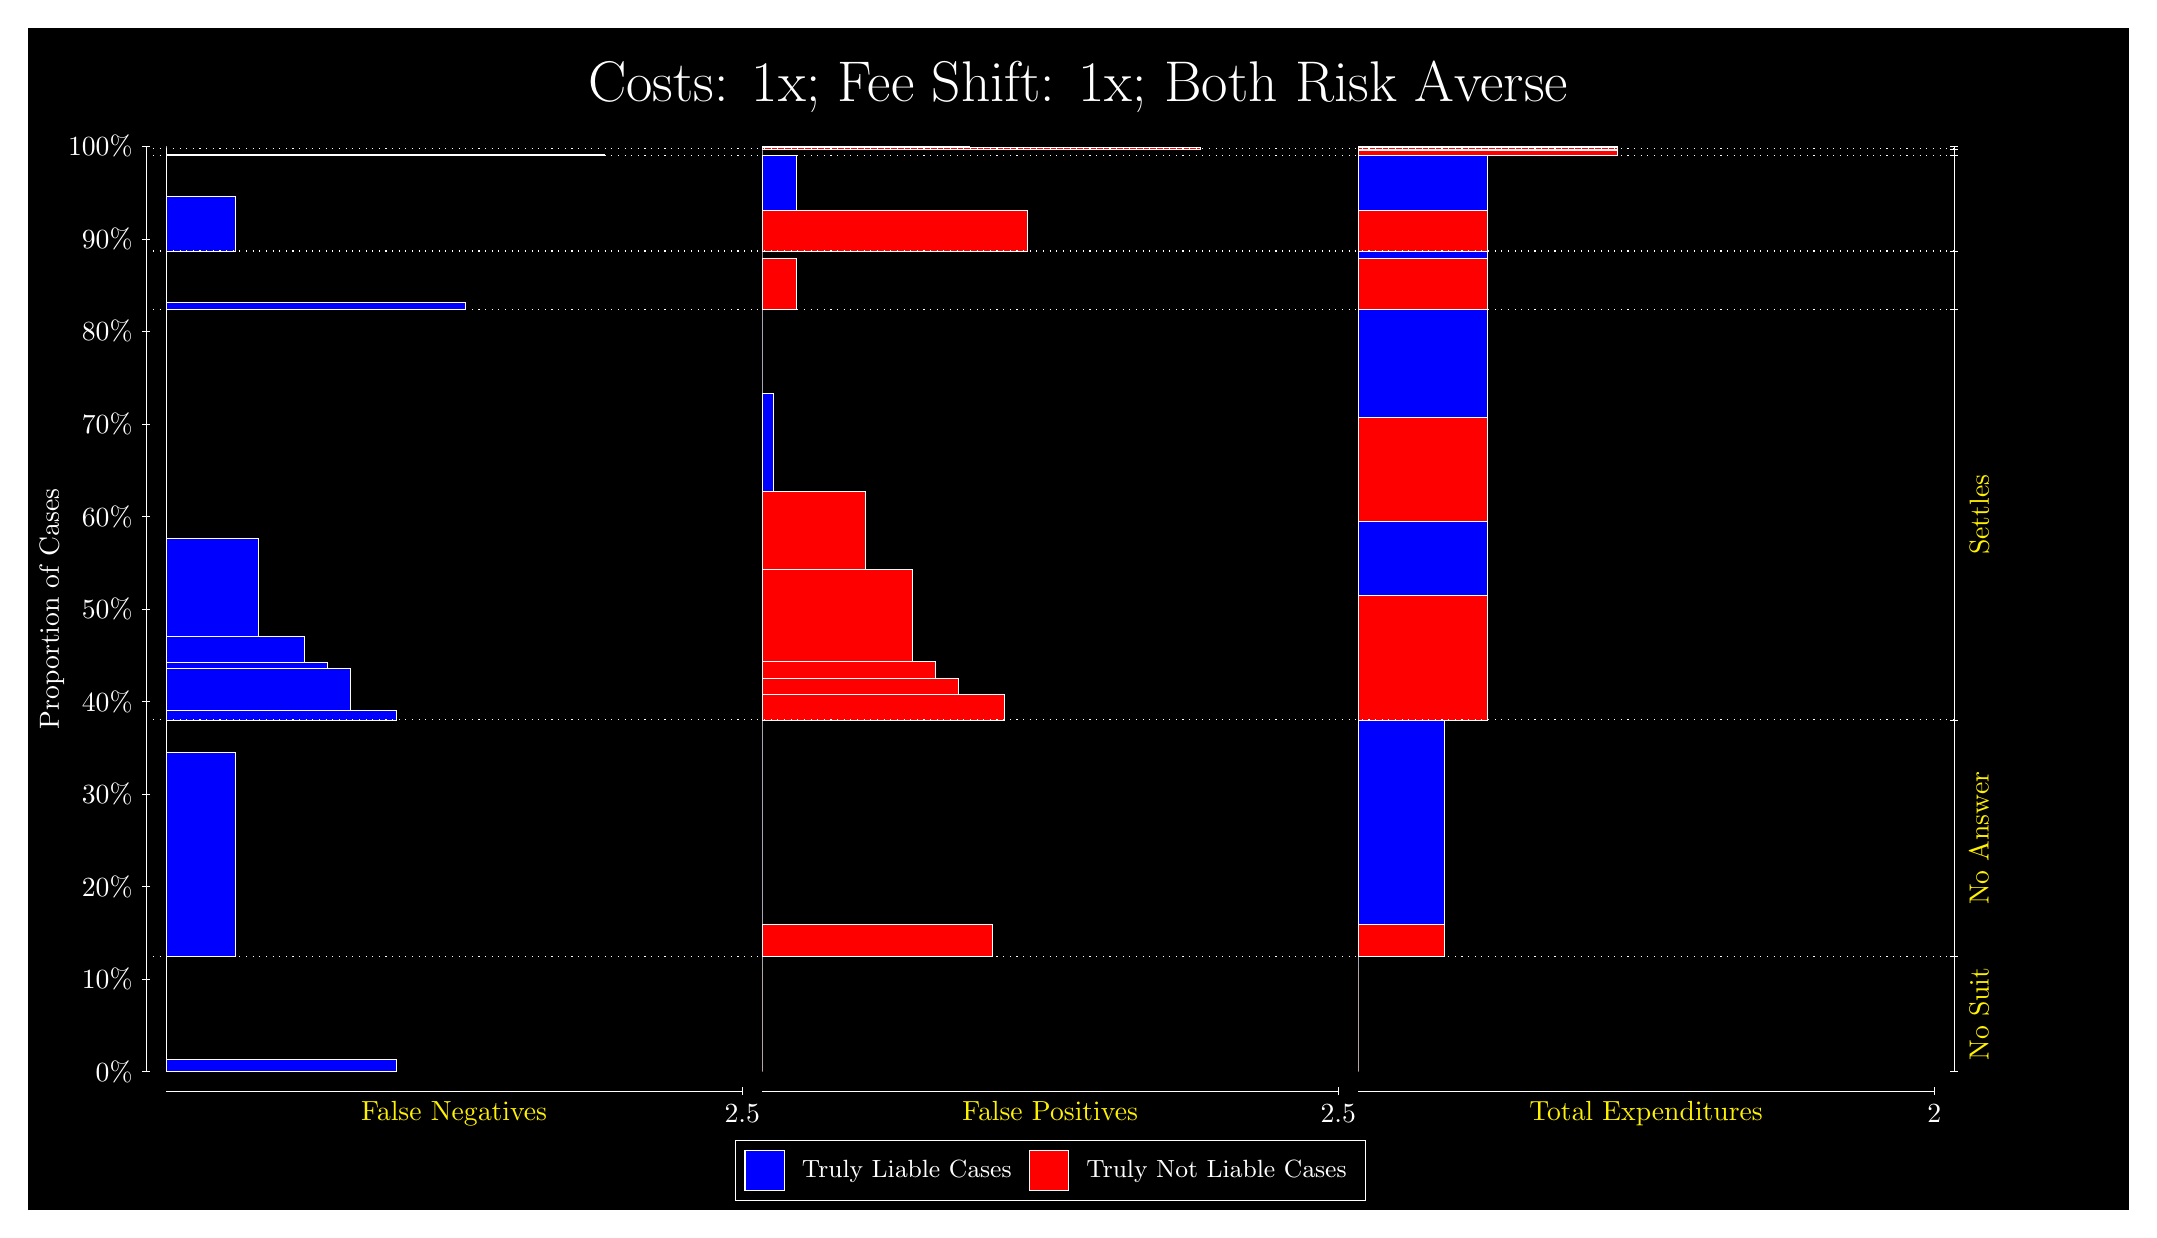
\begin{tikzpicture}
\draw[fill=black] (0,0) rectangle (26.667,15);
\draw[text=white] (0,13.5) rectangle (26.667,15) node[midway] {\huge Costs: 1x; Fee Shift: 1x; Both Risk Averse};
\draw[white, very thin] (1.5,1.75) -- (1.5,13.5);
\node[rotate=90, text=white, anchor=center] at (0.3, 7.625) {Proportion of Cases};
\draw[white, very thin] (1.45,1.75) -- (1.55,1.75);
\node[text=white, anchor=east] at (1.45, 1.75) {0\%};
\draw[white, very thin] (1.45,2.925) -- (1.55,2.925);
\node[text=white, anchor=east] at (1.45, 2.925) {10\%};
\draw[white, very thin] (1.45,4.1) -- (1.55,4.1);
\node[text=white, anchor=east] at (1.45, 4.1) {20\%};
\draw[white, very thin] (1.45,5.275) -- (1.55,5.275);
\node[text=white, anchor=east] at (1.45, 5.275) {30\%};
\draw[white, very thin] (1.45,6.45) -- (1.55,6.45);
\node[text=white, anchor=east] at (1.45, 6.45) {40\%};
\draw[white, very thin] (1.45,7.625) -- (1.55,7.625);
\node[text=white, anchor=east] at (1.45, 7.625) {50\%};
\draw[white, very thin] (1.45,8.8) -- (1.55,8.8);
\node[text=white, anchor=east] at (1.45, 8.8) {60\%};
\draw[white, very thin] (1.45,9.975) -- (1.55,9.975);
\node[text=white, anchor=east] at (1.45, 9.975) {70\%};
\draw[white, very thin] (1.45,11.15) -- (1.55,11.15);
\node[text=white, anchor=east] at (1.45, 11.15) {80\%};
\draw[white, very thin] (1.45,12.325) -- (1.55,12.325);
\node[text=white, anchor=east] at (1.45, 12.325) {90\%};
\draw[white, very thin] (1.45,13.5) -- (1.55,13.5);
\node[text=white, anchor=east] at (1.45, 13.5) {100\%};

\draw[white, very thin] (24.457,1.75) -- (24.457,13.5);
\draw[white, very thin] (24.407,1.75) -- (24.507,1.75);
\node[anchor=west] at (24.407, 1.75) {};
\draw[white, very thin] (24.407,3.2075) -- (24.507,3.2075);
\node[anchor=west] at (24.407, 3.2075) {};
\draw[white, very thin] (24.407,6.2151) -- (24.507,6.2151);
\node[anchor=west] at (24.407, 6.2151) {};
\draw[white, very thin] (24.407,11.429) -- (24.507,11.429);
\node[anchor=west] at (24.407, 11.429) {};
\draw[white, very thin] (24.407,12.17) -- (24.507,12.17);
\node[anchor=west] at (24.407, 12.17) {};
\draw[white, very thin] (24.407,13.383) -- (24.507,13.383);
\node[anchor=west] at (24.407, 13.383) {};
\draw[white, very thin] (24.407,13.467) -- (24.507,13.467);
\node[anchor=west] at (24.407, 13.467) {};
\draw[white, very thin] (24.407,13.5) -- (24.507,13.5);
\node[anchor=west] at (24.407, 13.5) {};

\draw[white, very thin, fill=blue] (1.75,1.75) rectangle (4.6775,1.9033);
\draw[white, very thin, fill=red] (1.75,1.9033) rectangle (1.75,3.2075);
\draw[white, very thin, fill=blue] (1.75,3.2075) rectangle (2.6283,5.7984);
\draw[white, very thin, fill=red] (1.75,5.7984) rectangle (1.75,6.2151);
\draw[white, very thin, fill=blue] (1.75,6.2151) rectangle (4.6775,6.3325);
\draw[white, very thin, fill=blue] (1.75,6.3325) rectangle (4.092,6.8672);
\draw[white, very thin, fill=blue] (1.75,6.8672) rectangle (3.7993,6.9414);
\draw[white, very thin, fill=blue] (1.75,6.9414) rectangle (3.5065,7.276);
\draw[white, very thin, fill=blue] (1.75,7.276) rectangle (2.921,8.5269);
\draw[white, very thin, fill=red] (1.75,8.5269) rectangle (1.75,11.429);
\draw[white, very thin, fill=blue] (1.75,11.429) rectangle (5.5558,11.518);
\draw[white, very thin, fill=red] (1.75,11.518) rectangle (1.75,12.17);
\draw[white, very thin, fill=blue] (1.75,12.17) rectangle (2.6283,12.866);
\draw[white, very thin, fill=red] (1.75,12.866) rectangle (1.75,13.383);
\draw[white, very thin, fill=blue] (1.75,13.383) rectangle (7.3123,13.4);
\draw[white, very thin, fill=red] (1.75,13.4) rectangle (1.75,13.467);
\draw[white, very thin, fill=red] (1.75,13.467) rectangle (1.75,13.484);
\draw[white, very thin, fill=blue] (1.75,13.484) rectangle (1.75,13.5);
\draw[white, very thin, fill=red] (9.3189,1.75) rectangle (9.3189,3.0542);
\draw[white, very thin, fill=blue] (9.3189,3.0542) rectangle (9.3189,3.2075);
\draw[white, very thin, fill=red] (9.3189,3.2075) rectangle (12.246,3.6242);
\draw[white, very thin, fill=blue] (9.3189,3.6242) rectangle (9.3189,6.2151);
\draw[white, very thin, fill=red] (9.3189,6.2151) rectangle (12.393,6.5469);
\draw[white, very thin, fill=red] (9.3189,6.5469) rectangle (11.807,6.7446);
\draw[white, very thin, fill=red] (9.3189,6.7446) rectangle (11.515,6.9572);
\draw[white, very thin, fill=red] (9.3189,6.9572) rectangle (11.222,8.1264);
\draw[white, very thin, fill=red] (9.3189,8.1264) rectangle (10.636,9.1168);
\draw[white, very thin, fill=blue] (9.3189,9.1168) rectangle (9.4652,10.368);
\draw[white, very thin, fill=blue] (9.3189,10.368) rectangle (9.3189,11.429);
\draw[white, very thin, fill=red] (9.3189,11.429) rectangle (9.758,12.081);
\draw[white, very thin, fill=blue] (9.3189,12.081) rectangle (9.3189,12.17);
\draw[white, very thin, fill=red] (9.3189,12.17) rectangle (12.686,12.686);
\draw[white, very thin, fill=blue] (9.3189,12.686) rectangle (9.758,13.383);
\draw[white, very thin, fill=red] (9.3189,13.383) rectangle (9.3189,13.449);
\draw[white, very thin, fill=blue] (9.3189,13.449) rectangle (9.3189,13.467);
\draw[white, very thin, fill=red] (9.3189,13.467) rectangle (14.881,13.484);
\draw[white, very thin, fill=blue] (9.3189,13.484) rectangle (11.954,13.5);
\draw[white, very thin, fill=red] (16.888,1.75) rectangle (16.888,3.0542);
\draw[white, very thin, fill=blue] (16.888,3.0542) rectangle (16.888,3.2075);
\draw[white, very thin, fill=red] (16.888,3.2075) rectangle (17.986,3.6242);
\draw[white, very thin, fill=blue] (16.888,3.6242) rectangle (17.986,6.2151);
\draw[white, very thin, fill=red] (16.888,6.2151) rectangle (18.534,7.7946);
\draw[white, very thin, fill=blue] (16.888,7.7946) rectangle (18.534,8.738);
\draw[white, very thin, fill=red] (16.888,8.738) rectangle (18.534,10.06);
\draw[white, very thin, fill=blue] (16.888,10.06) rectangle (18.534,11.429);
\draw[white, very thin, fill=red] (16.888,11.429) rectangle (18.534,12.081);
\draw[white, very thin, fill=blue] (16.888,12.081) rectangle (18.534,12.17);
\draw[white, very thin, fill=red] (16.888,12.17) rectangle (18.534,12.686);
\draw[white, very thin, fill=blue] (16.888,12.686) rectangle (18.534,13.383);
\draw[white, very thin, fill=red] (16.888,13.383) rectangle (20.181,13.449);
\draw[white, very thin, fill=blue] (16.888,13.449) rectangle (20.181,13.467);
\draw[white, very thin, fill=red] (16.888,13.467) rectangle (20.181,13.484);
\draw[white, very thin, fill=blue] (16.888,13.484) rectangle (20.181,13.5);
\draw[white, dotted] (1.5,3.2075) -- (24.457,3.2075);
\draw[white, dotted] (1.5,6.2151) -- (24.457,6.2151);
\draw[white, dotted] (1.5,11.429) -- (24.457,11.429);
\draw[white, dotted] (1.5,12.17) -- (24.457,12.17);
\draw[white, dotted] (1.5,13.383) -- (24.457,13.383);
\draw[white, dotted] (1.5,13.467) -- (24.457,13.467);
\draw[white, very thin] (1.75,1.5) -- (9.0689,1.5);
\node[text=yellow, anchor=north] at (5.4094, 1.5) {False Negatives};
\draw[white, very thin] (9.0689,1.45) -- (9.0689,1.55);
\node[text=white, anchor=north] at (9.0689, 1.45) {2.5};

\draw[white, very thin] (9.3189,1.5) -- (16.638,1.5);
\node[text=yellow, anchor=north] at (12.978, 1.5) {False Positives};
\draw[white, very thin] (16.638,1.45) -- (16.638,1.55);
\node[text=white, anchor=north] at (16.638, 1.45) {2.5};

\draw[white, very thin] (16.888,1.5) -- (24.207,1.5);
\node[text=yellow, anchor=north] at (20.547, 1.5) {Total Expenditures};
\draw[white, very thin] (24.207,1.45) -- (24.207,1.55);
\node[text=white, anchor=north] at (24.207, 1.45) {2};

\node[text=yellow, centered, rotate=90] at (24.777, 2.4788) {No Suit};
\node[text=yellow, centered, rotate=90] at (24.777, 4.7113) {No Answer};
\node[text=yellow, centered, rotate=90] at (24.777, 8.8218) {Settles};





\draw (12.978300999999998,1.5) node[draw=none] (baseCoordinate) {};
\begin{scope}[align=center]
        \matrix[scale=0.5, draw=white, below=0.5cm of baseCoordinate, nodes={draw}, column sep=0.1cm]{
            \node[rectangle, draw, minimum width=0.5cm, minimum height=0.5cm, fill=blue] {}; &
            \node[draw=none, font=\small, text=white] (B) {Truly Liable Cases}; &
            \node[rectangle, draw, minimum width=0.5cm, minimum height=0.5cm, fill=red] {}; &
            \node[draw=none, font=\small, text=white] (B) {Truly Not Liable Cases}; \\
            };
\end{scope}

\end{tikzpicture}
\end{document}